\documentclass[hyperref={pdfpagemode=FullScreen},aspectratio=169]{beamer}
\usetheme{CambridgeUS} % theme
\usepackage[english, italian]{babel}
\usepackage[utf8x]{inputenc}
\usepackage{ragged2e}

\setbeamercovered{transparent} % \pause text visibility
\beamertemplatenavigationsymbolsempty
\setbeamertemplate{frametitle}[default][center]
\setbeamerfont{title}{size=\huge}
\setbeamerfont{frametitle}{size=\huge}
\setbeamerfont{framesubtitle}{size=\huge}
\setbeamerfont{author}{size=\Large}
%\setbeamerfont{date}{size=\Large}
\setbeamerfont{institute}{size=\Large}
\addtobeamertemplate{block begin}{\pgfsetfillopacity{0.8}}{\pgfsetfillopacity{1}}
\setbeamercolor{structure}{fg=red} %colore pallini elenco puntato
\setbeamercolor{block title}{fg=white, bg= red}
\setbeamercolor*{block body}{bg= red!30}
\setbeamerfont{block title}{size=\Large}
\setbeamerfont{block body}{size=\Large}

%------------------------------ TITLE PAGE DECLARATION
\makeatletter
\newcommand\titlegraphicii[1]{\def\inserttitlegraphicii{#1}}
\titlegraphicii{}
\setbeamertemplate{title page}
{
  \begin{centering}
    \begin{beamercolorbox}[sep=8pt,center]{institute}
      \usebeamerfont{institute}\insertinstitute
    \end{beamercolorbox}
    \usebeamercolor[fg]{titlegraphic}\inserttitlegraphic\hfill\inserttitlegraphicii\par
    \vskip0.20em%
    \begin{beamercolorbox}[sep=8pt,center]{title}
      \usebeamerfont{title}\inserttitle\par%
      \ifx\insertsubtitle\@empty%
      \else%
        %\vskip0.25em%
        {\usebeamerfont{subtitle}\usebeamercolor[fg]{subtitle}\insertsubtitle\par}%
      \fi%     
    \end{beamercolorbox}%
    \vskip0.20em\par
    \begin{beamercolorbox}[sep=8pt,center]{author}
      \usebeamerfont{author}\insertauthor
    \end{beamercolorbox} \vskip-0.5em
%    \begin{beamercolorbox}[sep=8pt,center]{date}
%      \usebeamerfont{date}\insertdate
 %   \end{beamercolorbox}
  \end{centering}
  %\vfill
}
\makeatother
\author[14 dicembre 2016]{\textbf{Marco Prelaz \\1047343}}
\title[]{\textsc{Supporto e consulenza tecnica dell'applicativo NPS}}
\institute[]{Università degli Studi di Padova\\ \vskip0.2em 
\includegraphics[height=20pt]{images/logoDM}\\ Corso di Laurea in Informatica}
\date[]{Anno accademico 2015-2016}
%\logo{
\includegraphics[width=1cm]{images/logo_unipd}}
\titlegraphic{
\includegraphics[height=60pt]{images/logo_unipd}}
%------------------------------ /TITLE PAGE DECLARATION

\begin{document}

\frame{\titlepage}


%\section*{Indice dei contenuti}
%\begin{frame} %------------------------------ OUTLINE
%\frametitle{Indice dei contenuti}
%\tableofcontents
%\end{frame}

\section{}
\begin{frame}
\frametitle[centering]{MEDIANA}
\vspace{-30pt}
     \begin{columns}[T] % contents are top vertically aligned
     
     \begin{column}[T]{7cm} % each column can also be its own environment
     \begin{Large}
     \begin{center}
     \vskip1em
     Azienda che si occupa di fornire \textbf{soluzioni software} utili alla crescita di aziende legate soprattutto al settore dell'\textbf{energia elettrica} e del \textbf{gas}
     \end{center}
     \end{Large}     
     \end{column} 
     
     \begin{column}[T]{7cm} % alternative top-align that's better for graphics
     \begin{LARGE}
     \begin{center}
     
\includegraphics[height=45pt]{images/mediana_logo} \\ \vskip0.8em
    
\includegraphics[height=50pt]{images/electric} \hskip2em 
\includegraphics[height=50pt]{images/gas}
     \end{center}
     \end{LARGE} 
     \end{column}
     
     \end{columns}
\end{frame}

\section{}
\begin{frame}
\frametitle{IL CONCETTO ENPS}
\vspace{-10pt}
\begin{center}
\begin{Large}
\textit{Su una scala da 0 a 10, con quale probabilità consiglieresti \\ questa azienda come posto di lavoro?} \\ \vskip1em%
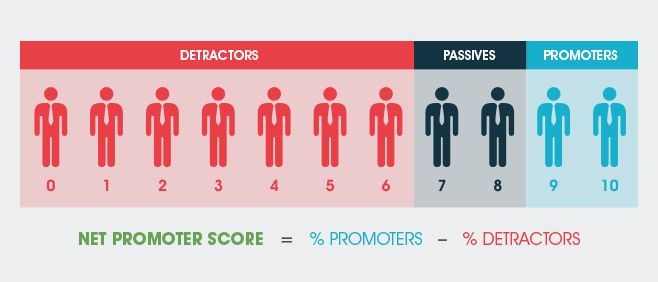
\includegraphics[height=120pt]{images/NPS} \\
\end{Large}
\end{center}
\end{frame}

\section{}
\begin{frame}
\frametitle{L'APPLICATIVO NPS EBS}
\vspace{-30pt}
\begin{center}

\includegraphics[height=60pt]{images/eon} 
\end{center}

\begin{block}{\begin{center}La richiesta\end{center}}
Applicativo in grado di gestire \textbf{web survey} utilizzabili per raccogliere i \textbf{feedback} necessari a calcolare l'\textbf{ENPS}
\end{block}
\end{frame}

\section{}
\begin{frame}
\frametitle{FUNZIONALITÀ PRINCIPALI}
\framesubtitle{Indagini}
\vspace{-30pt}
     \begin{columns}[T] % contents are top vertically aligned
     
\begin{column}[T]{7cm} % alternative top-align that's better for graphics
\begin{flushright}
\begin{Large}
 \vskip1.2em Caricamento anagrafiche dei dipendenti \\ 
 \vskip1.8em Selezione dei contatti \\ 
 \vskip2.7em Invio delle survey
\end{Large}
\end{flushright}
     \end{column}     
     
     \begin{column}[T]{7cm} % each column can also be its own environment
     \begin{center} \vskip1em
     
\includegraphics[height=35pt]{images/upload} \\ \vskip1.5em
     
\includegraphics[height=40pt]{images/contactSelection} \\ \vskip0.8em
     
\includegraphics[height=50pt]{images/mail} 
     \end{center}     
     \end{column} 
     
     \end{columns}
\end{frame}

\section{}
\begin{frame}
\frametitle{FUNZIONALITÀ PRINCIPALI}
\framesubtitle{Categorizzazione}
\vspace{-10pt}
\begin{columns}[T] % contents are top vertically aligned
     
     \begin{column}[T]{5cm} % each column can also be its own environment
     \begin{Large}
     \begin{center}
     
\includegraphics[height=40pt]{images/Like} \hskip0.2em 
\includegraphics[height=40pt]{images/Dislike} \hskip0.2em 
\includegraphics[height=40pt]{images/Idea} \\ \vskip1.5em \textbf{Type}
     \end{center}
     \end{Large}
     \end{column}
     
     \begin{column}[T]{5cm} % each column can also be its own environment
     \begin{Large}
     \begin{center}
     
\includegraphics[height=40pt]{images/ProblemiComunicazione} \hskip0.2em 
\includegraphics[height=40pt]{images/ProblemiSoftware} \hskip0.2em 
\includegraphics[height=40pt]{images/ProblemiHardware} \\ \vskip1.5em \textbf{Class}
     \end{center}
     \end{Large}
     \end{column}
     
     \begin{column}[T]{5cm} % each column can also be its own environment
     \begin{Large}
     \begin{center}
     
\includegraphics[height=40pt]{images/Laptop} \hskip0.2em 
\includegraphics[height=40pt]{images/PC} \hskip0.2em 
\includegraphics[height=40pt]{images/Smartphone} \\ \vskip1.5em \textbf{Topic}
     \end{center}
     \end{Large}
     \end{column}
     
\end{columns}
\end{frame}


\section{}
\begin{frame}
\frametitle{FUNZIONALITÀ PRINCIPALI}
\framesubtitle{Reportistica}
\vspace{-30pt}
     \begin{columns}[T] % contents are top vertically aligned
     
     \begin{column}[T]{7cm} % each column can also be its own environment
     \begin{center} \vskip0.8em
     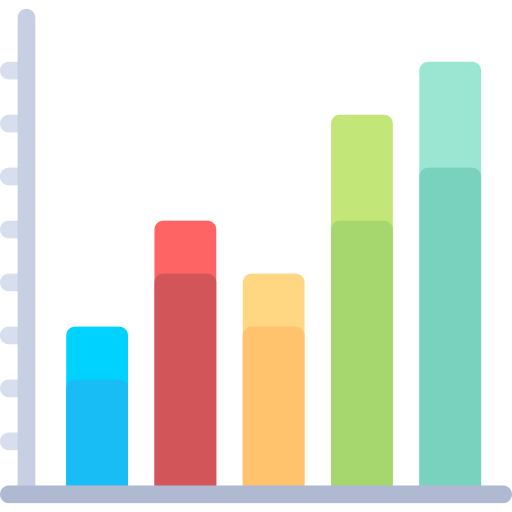
\includegraphics[height=50pt]{images/Barre} \\ \vskip0.8em
     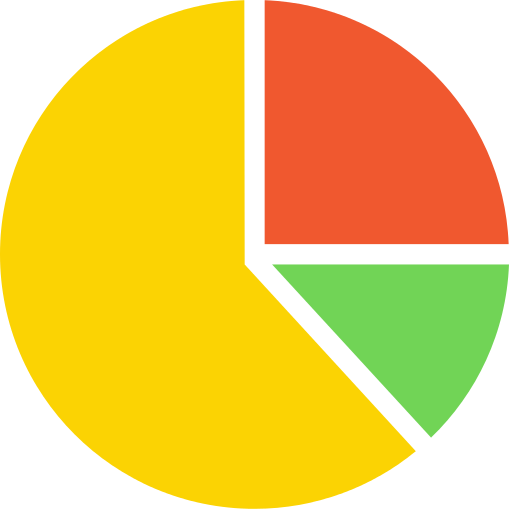
\includegraphics[height=40pt]{images/Torta} \\ \vskip0.8em
     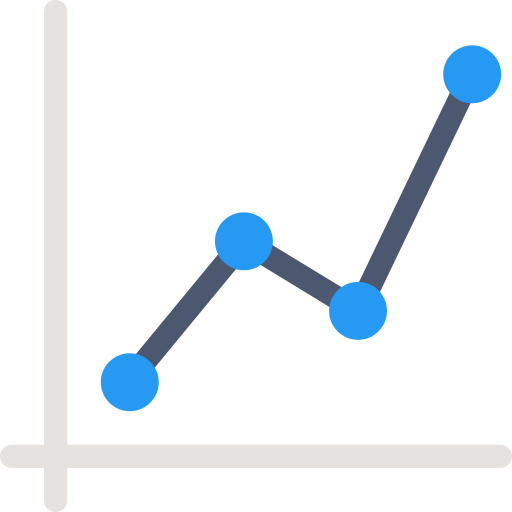
\includegraphics[height=50pt]{images/Linee} 
     \end{center}     
     \end{column} 
     
     \begin{column}[T]{7cm} % alternative top-align that's better for graphics
     \begin{Large}
      \vskip2.6em \textbf{Grafici a barre} per analizzare la distribuzione  \\ 
 \vskip1.2em \textbf{Grafici a torta} per avere una visione d'insieme  \\ 
 \vskip1.7em \textbf{Grafici a linee} per analizzare l'andamento temporale 
     \end{Large}
     \end{column}
     
     \end{columns}
\end{frame}

\section{}
\begin{frame}
\frametitle{FUNZIONALITÀ PRINCIPALI}
\framesubtitle{Iniziative}
\vspace{-30pt}
\begin{center}
\begin{Large}
Azione intrapresa con lo scopo di migliorare \\ la soddisfazione dell'organico aziendale
\end{Large}
\end{center}
\begin{columns}[T] % contents are top vertically aligned
     
     \begin{column}[T]{5cm} % each column can also be its own environment
     \begin{flushright}
     
\includegraphics[height=50pt]{images/sad}
     \end{flushright}
     \end{column}
     
     \begin{column}[T]{5cm} % each column can also be its own environment
     \begin{center}
     
\includegraphics[height=50pt]{images/arrow}
     \end{center}
     \end{column}
     
     \begin{column}[T]{5cm} % each column can also be its own environment
     \begin{flushleft}
     
\includegraphics[height=50pt]{images/happy}
     \end{flushleft}
     \end{column}
     
\end{columns}

\end{frame}



\section{}
\begin{frame}
\frametitle{OBIETTIVI}
\vspace{-5pt}
\begin{Large}
\begin{center}
\begin{itemize}
  \item Conoscenza degli applicativi di Mediana, in particolare di NPS \vskip0.8em
  \item Conoscenza delle fasi consulenziali: \vskip0.4em
  	\begin{itemize}
  	\item Redazione di test book per U.A.T. \vskip0.8em
  	\item Test e verifiche dei programmi presi in esame \vskip0.8em
  	\item Redazione di manuali propedeutici al roll out dell'applicativo \vskip0.8em
  	\end{itemize} 
  \item Apprendimento del data model di NPS EBS \vskip0.8em
  \item Sviluppare una buona autonomia nella progettazione e sviluppo di statement
SQL
\end{itemize}
\end{center}
\end{Large}
\end{frame}

\section{}
\begin{frame}
\frametitle{CONSULENTE}
\framesubtitle{Fasi di un progetto}
\vspace{-10pt}
\begin{center}
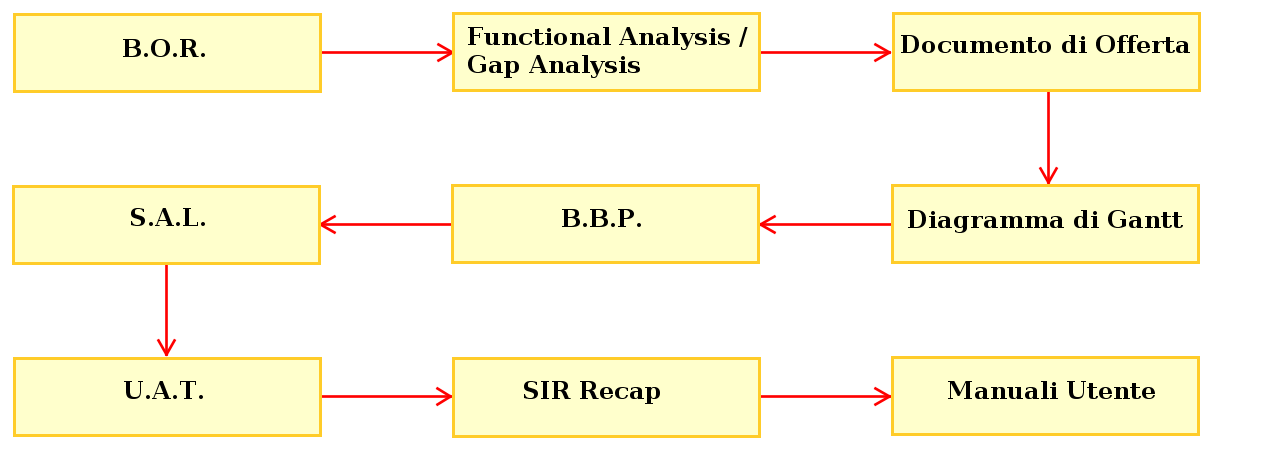
\includegraphics[height=160pt]{images/FasiProgetto}
\end{center}
\end{frame}

\section{}
\begin{frame}
\frametitle{CONSULENTE}
\framesubtitle{Attività svolte}
\vspace{-10pt}
\begin{columns}[T] % contents are top vertically aligned

\begin{column}[T]{11cm} % alternative top-align that's better for graphics
\begin{Large}
\begin{center}
\begin{itemize}
  \item Studio documentazione chiave di NPS EBS: \vskip0.4em
  	\begin{itemize}
  	\item B.O.R. del progetto originale \vskip0.8em
  	\item B.B.P. sprint 3 \vskip0.8em
  	\end{itemize} 
  \item Test di accettazione dell'applicativo \\ e issue tracking \vskip0.8em
  \item Aggiornamento manuali utente con le funzionalità nuove/modificate
\end{itemize}
\end{center}
\end{Large}
\end{column}

\begin{column}[T]{3cm} % alternative top-align that's better for graphics
     \begin{LARGE}
     \begin{center}
     \vskip60pt
     
\includegraphics[height=40pt]{images/GoogleDrive} \\ \vskip0.8em
    
\includegraphics[height=40pt]{images/Word}
     \end{center}
     \end{LARGE} 
     \end{column}
     
\end{columns}
\end{frame}

\section{}
\begin{frame}
\frametitle{SVILUPPATORE}
\framesubtitle{Tecnologie utilizzate}
\vspace{-10pt}
     \begin{columns}[T] % contents are top vertically aligned
     
     \begin{column}[T]{4cm} % each column can also be its own environment
     \begin{LARGE}
     \begin{center}
     
\includegraphics[height=50pt]{images/visualStudio} \\ \vskip1.5em
      
\includegraphics[height=50pt]{images/cSharp} 
     \end{center}
     \end{LARGE}     
     \end{column} 
     
     \begin{column}[T]{4cm} % alternative top-align that's better for graphics
     \begin{LARGE}
     \begin{center}
     
\includegraphics[height=50pt]{images/aspNet}\\ \vskip1.5em
    
\includegraphics[height=50pt]{images/VSS}
     \end{center}
     \end{LARGE} 
     \end{column}
     
     \begin{column}[T]{4cm} % alternative top-align that's better for graphics
     \begin{LARGE}
     \begin{center}
     
\includegraphics[height=50pt]{images/sqlServer} \\ \vskip1.5em
    
\includegraphics[height=50pt]{images/TSQL} 
     \end{center}
     \end{LARGE} 
     \end{column}
     
     \end{columns}
\end{frame}

\section{}
\begin{frame}
\frametitle{SVILUPPATORE}
\framesubtitle{Attività svolte}
\vspace{-10pt}
\begin{block}{\begin{center}Support NPS EBS\end{center}}
\begin{columns}[T] % contents are top vertically aligned
     
     \begin{column}[T]{5cm} % each column can also be its own environment
     \begin{center}
     
\includegraphics[height=50pt]{images/BugFix} 
     \end{center}     
     \end{column} 
     
     \begin{column}[T]{5cm} % each column can also be its own environment
     \begin{center}
     
\includegraphics[height=50pt]{images/Excel} 
     \end{center}     
     \end{column} 
     
      \begin{column}[T]{5cm} % each column can also be its own environment
     \begin{center}
     
\includegraphics[height=50pt]{images/DB} 
     \end{center}     
     \end{column} 
     
     \end{columns}
\end{block}
\end{frame}

\section{}
\begin{frame}
\frametitle{PIANO DI LAVORO}
\vspace{-20pt}
\begin{center}
     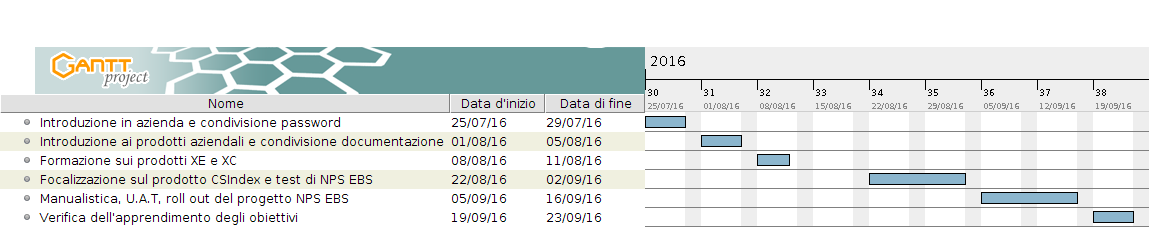
\includegraphics[height=80pt]{images/GanttPianificazione} 
     \end{center}  
\begin{block}{Cause delle differenze rispetto alla pianificazione:}
\begin{Large}
\begin{center}
\begin{itemize} \vskip0.2em
  \item Rischio non calcolabile \vskip0.4em
  \item Pianificazione troppo generica \vskip0.4em
  \item Attività sovrastimate 
\end{itemize}
\end{center}
\end{Large}
\end{block}
\vspace{-10pt}

\end{frame}

\section{}
\begin{frame}
\frametitle{CONCLUSIONI}
\vspace{-10pt}
\begin{columns}[T] % contents are top vertically aligned
     
     \begin{column}[T]{5cm} % each column can also be its own environment
     \begin{Large}
     \begin{center}
     
\includegraphics[height=50pt]{images/Obiettivi} \\ \vskip1.5em \textbf{Obiettivi nel complesso raggiunti}
     \end{center}
     \end{Large}
     \end{column}
     
     \begin{column}[T]{5cm} % each column can also be its own environment
     \begin{Large}
     \begin{center}
     
\includegraphics[height=50pt]{images/Ampliare} \\ \vskip1.5em \textbf{Ampliamento conoscenze tecniche e professionali}
     \end{center}
     \end{Large}
     \end{column}
     
     \begin{column}[T]{5cm} % each column can also be its own environment
     \begin{Large}
     \begin{center}
     
\includegraphics[height=50pt]{images/Positiva}  \\ \vskip1.5em \textbf{Valutazione dello stage positiva}
     \end{center}
     \end{Large}
     \end{column}
     
\end{columns}
\end{frame}

\section{}
\begin{frame}
\frametitle{}
\begin{Huge}
\begin{center}
\textsc{Grazie per l'attenzione}
\end{center}
\end{Huge}
\end{frame}

\end{document}